\chapter{Descripción de realización}

\section{Método de desarrollo}

El proyecto se desarrollará mediante un sistema de fases, en las que el orden es algo vital puesto que cada una de las fases dependerá de la previa. Por tanto, las fases de la solución planteada serán las siguientes:

\begin{enumerate}
	\item \textbf{Análisis de las herramientas a usar:}

	En esta fase se analizarán todas las posibles herramientas que se pueden usar para el desarrollo del proyecto y se elegirán las más adecuadas de acuerdo a las necesidades del proyecto y a los conocimientos del equipo de trabajo.
	\item \textbf{Integración y modelado de datos:}

	Es la fase en la que se identificará y seleccionarán las tablas del repositorio de las que se extraerá la información para su adaptación a Dublin Core.
	\item \textbf{Creación del servidor de OAI-PMH:}

	Diseño e implementación servidor.
	\item \textbf{Creación de la aplicación web:}

	Diseño e implementación del front-end de la aplicación web. 
	\item \textbf{Validación técnica y de usabilidad:}

	Es la fase donde se realizarán las pruebas finales del sistema completo.
	\item \textbf{Documentación y despliegue en producción:}

	Es donde se terminará de redactar la documentación necesaria y se desplegará el producto.
\end{enumerate}

\subsection{Productos intermedios}

Los productos intermedios que se generarán en cada una de las fases son:

\begin{itemize}
	\item \textbf{Integración y modelado de datos:}
	\begin{itemize}
		\item Especificación y diseño de la base de conocimiento del servidor OAI-PMH.
	\end{itemize}
	\item \textbf{Creación parte servidora del sistema:}
	\begin{itemize}
		\item Módulo de proveedor de la base de conocimiento.
		\item Módulo de adaptación y almacenamiento del conocimiento en Dublin Core.
		\item Módulo de servicio de XMLs.
	\end{itemize}
	\item \textbf{Creación de la aplicación web:}
	\begin{itemize}
		\item Aplicación web del sistema.
	\end{itemize}
	\item \textbf{Validación técnica y de usabilidad:}
	\begin{itemize}
		\item Informe de evaluación del sistema
	\end{itemize}
\end{itemize}

\subsection{EDT}

\begin{figure}[!htp]
	\centering
	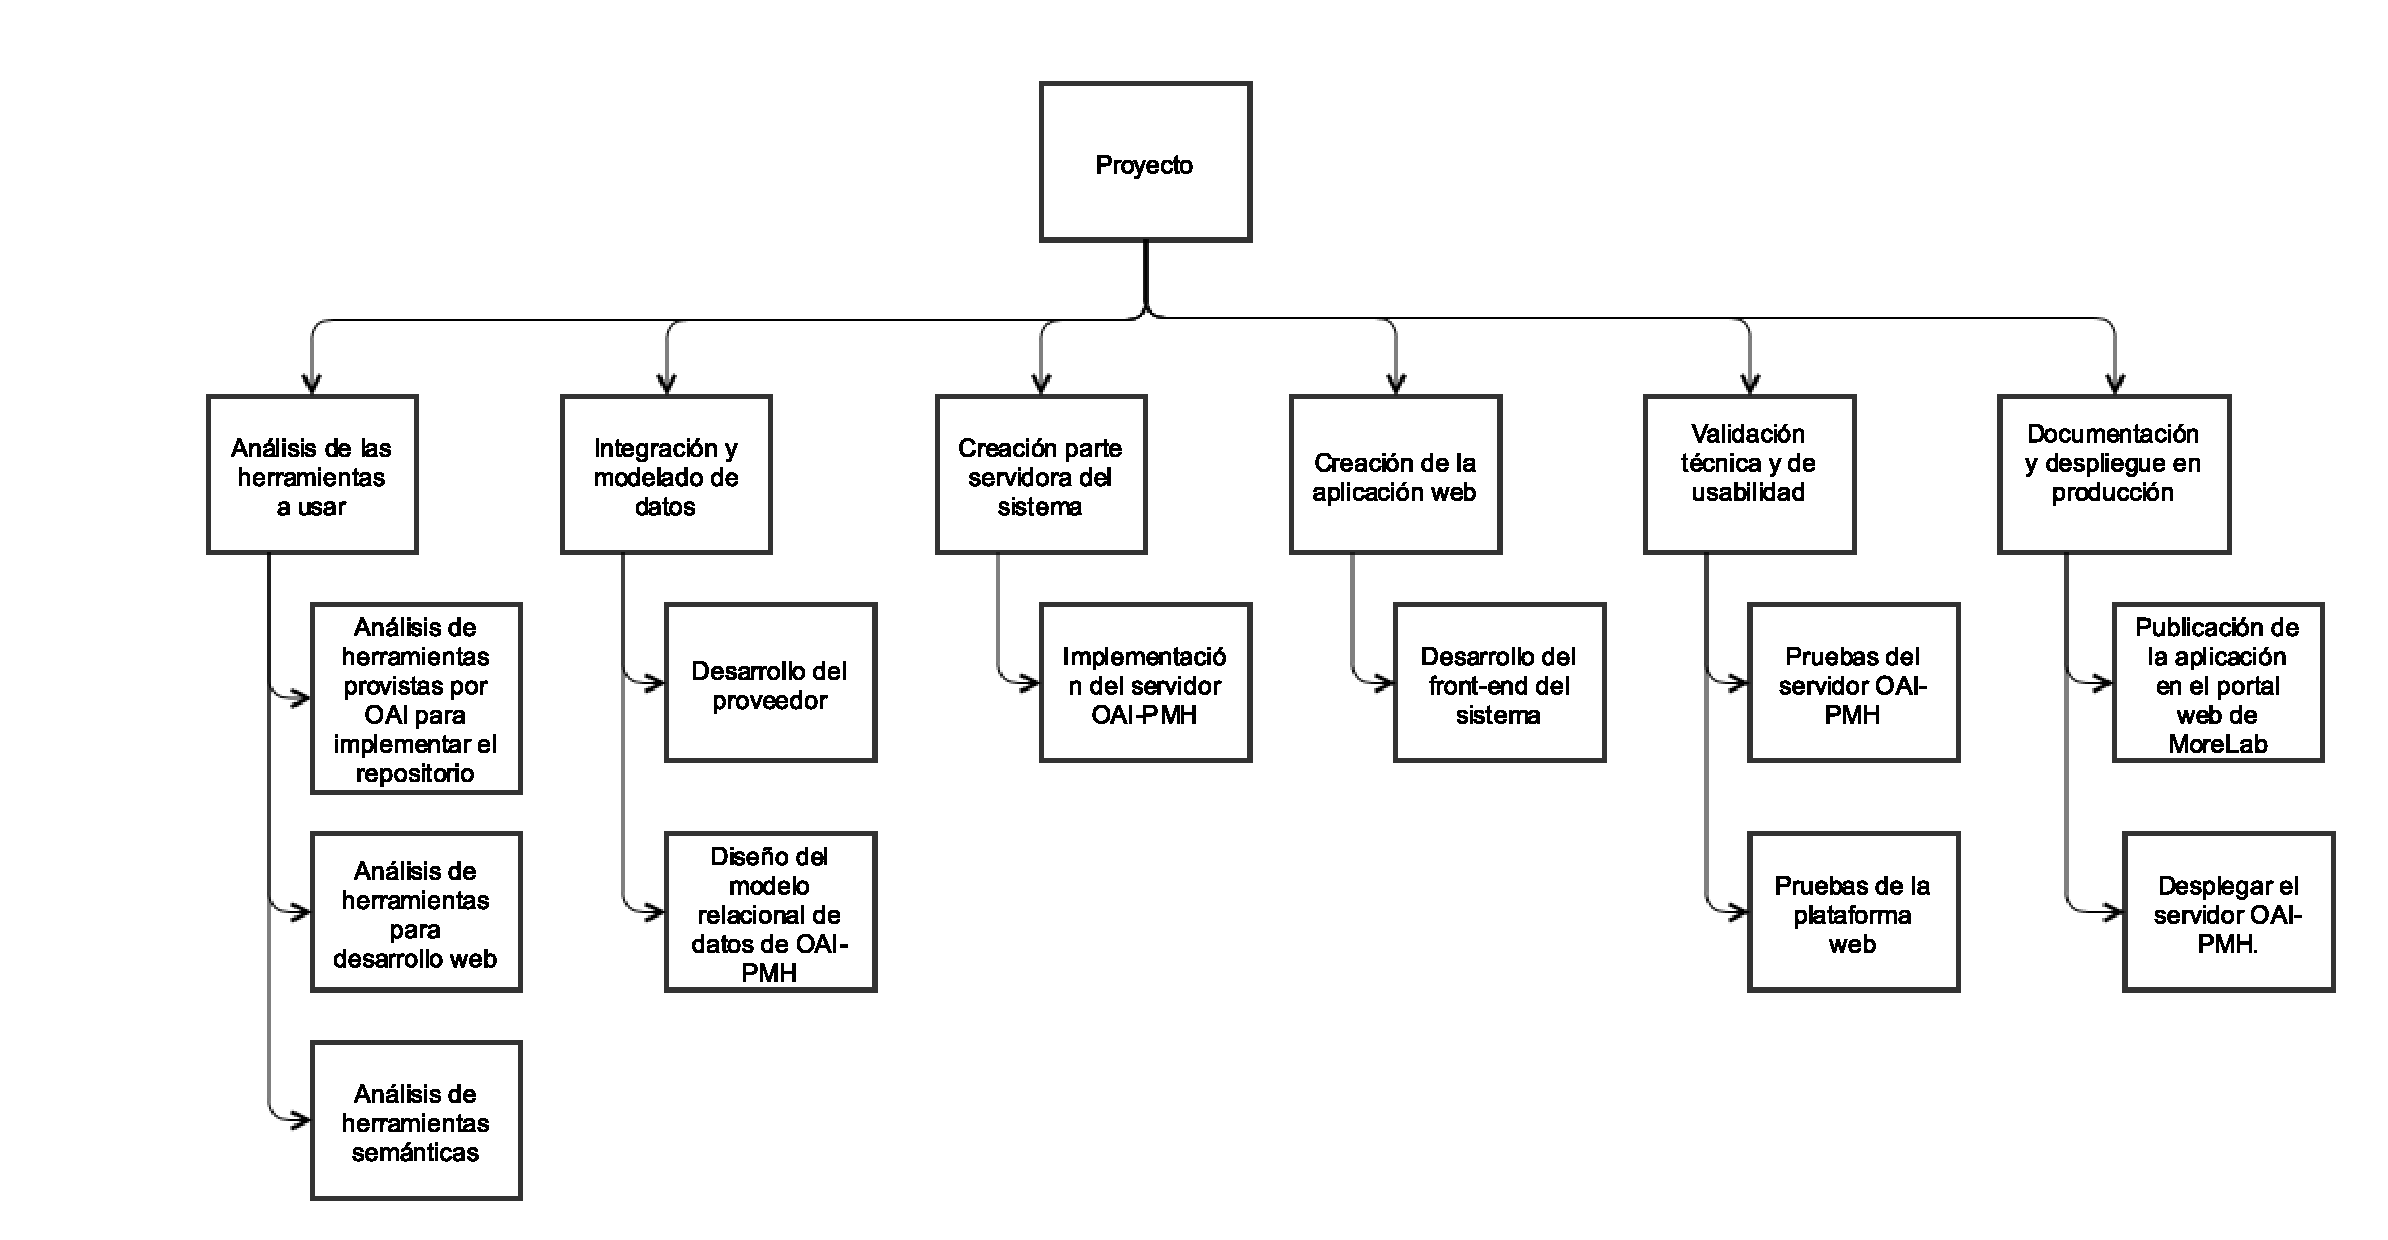
\includegraphics[angle=-90, scale=.5]{fig/edt}
	\caption{EDT}
\end{figure}

\section{Tareas principales}

La implantación del proyecto comprende las siguientes tareas o actividades: 

\subsection{Análisis de las herramientas a usar:}

\begin{itemize}
	\item \textbf{Análisis de herramientas provistas por OAI para implementar los requisitos mínimos para repositorio del protocolo OAI-PMH.}

	Investigar las distintas alternativas que hay para crear un servidor que beba de distintos tipos repositorios.
	\item \textbf{Análisis de herramientas para desarrollo web.}

	Investigar las distintas herramientas que hay para el desarrollo web y que sean adecuadas para el propósito del proyecto.
	\item \textbf{Análisis de herramientas semánticas.}

	Investigar las distintas alternativas para realizar búsquedas según los estándares de la web semántica. 
\end{itemize}

\subsection{Integración y modelado de datos:}

\begin{itemize}
	\item \textbf{Desarrollo del proveedor.}
	
	Desarrollo del sistema de extracción de datos de las tablas necesarias del repositorio PostgreSQL.

	\begin{enumerate}
		\item Formación: aprendizaje en el uso de las herramientas.
		\item Diseño: diseño del sistema de extracción de datos.
		\item Implementación: programación del sistema de extracción de datos.
		\item Pruebas: pruebas del sistema de extracción de datos.
	\end{enumerate}
	\item \textbf{Diseño del modelo relacional de datos de OAI-PMH.}
	\begin{enumerate}
		\item Diseño: diseño del modelo de la base de datos. 
		\item Implementación: inserción del modelo de datos en la base de datos.
		\item Pruebas: pruebas de la base de datos junto con el sistema de extracción de datos.
	\end{enumerate}
\end{itemize}

\subsection{Creación parte servidora del sistema:}

\begin{itemize}
	\item Implementación del servidor OAI-PMH.

	Puesta en marcha del servidor OAI-PMH que transforma datos almacenados mediante un modelo relacional a Dublin Core.

	\begin{enumerate}
		\item Implementación: configuración del servidor.
		\item Pruebas: pruebas del servidor.
	\end{enumerate}
\end{itemize}

\subsection{Creación de la aplicación web:}

\begin{itemize}
	\item \textbf{Desarrollo del front-end del sistema.}
	\begin{enumerate}
		\item Formación en la herramienta de desarrollo web.
		\item Diseño básico de la plataforma web.
		\item Diseño del módulo de búsquedas semánticas.
		\item Diseño del módulo de búsquedas facetadas.
	\end{enumerate}	
\end{itemize}

\subsection{Validación técnica y de usabilidad:}

\begin{itemize}
	\item \textbf{Pruebas del servidor OAI-PMH.}
	\item \textbf{Pruebas de la plataforma web.}
\end{itemize}

\subsection{Documentación y despliegue en producción:}

\begin{itemize}
	\item \textbf{Publicación de la aplicación en el portal web de MoreLab.}
	
	Instalar la aplicación web en el servidor de LabMan y publicarlo en el portal web.
	\item \textbf{Desplegar el servidor OAI-PMH.}

	Instalar el servidor OAI-PMH, recolectar y exportar la información del repositorio.
\end{itemize}

\section{Hoja de Tareas}

% Tarea 1 %

\begin{center}
	\begin{tabularx}{\textwidth}{@{\extracolsep{\fill} } | X | X | X |}
	\noalign{\hrule height 4pt}
	\multicolumn{3}{!{\vrule width 4pt} c !{\vrule width 4pt}}{\textbf{HOJA DE TAREAS}}	\\ \noalign{\hrule height 2pt}
	\multicolumn{3}{!{\vrule width 4pt} l !{\vrule width 4pt}}{\textbf{Nombre:} Jesus Sesma Solance}	\\
	\multicolumn{3}{!{\vrule width 4pt} l !{\vrule width 4pt}}{\textbf{Fecha:} Marzo de 2015}			\\	\noalign{\hrule height 2pt}
	\multicolumn{2}{!{\vrule width 4pt} l}{\textbf{Identificación de Tarea:} T1}	&
		\multicolumn{1}{!{\vrule width 2pt} l !{\vrule width 4pt}}{\textbf{Duración:} 3 días}	\\	\Cline{2pt}{3-3}
	\multicolumn{2}{!{\vrule width 4pt} l}{\textbf{Descripción:}}	&
		\multicolumn{1}{!{\vrule width 2pt} l !{\vrule width 4pt}}{\textbf{Esfuerzo:} 56 horas}	\\
	\multicolumn{2}{!{\vrule width 4pt} p{0.7\linewidth}}{Investigar las distintas alternativas que hay para crear un servidor que   beba de distintos tipos de repositorios. Principalmente de las herramientas registradas en la página de especificación del protocolo de OAI. Analizar la viabilidad de adaptación de dichas herramientas para ajustarla especialmente para el repositorio de LabMan. En caso contrario, realizar un estudio del protocolo para la futura implementación del protocolo completo.} &
		\multicolumn{1}{!{\vrule width 2pt} l !{\vrule width 4pt}}{}	\\	\noalign{\hrule height 2pt} 
	\multicolumn{2}{!{\vrule width 4pt} l}{\textbf{Criterios de Terminación:}}	&
		\multicolumn{1}{!{\vrule width 2pt} l !{\vrule width 4pt}}{\textbf{Tareas previas:}}	\\
	\multicolumn{2}{!{\vrule width 4pt} p{0.7\linewidth}}{La tarea se considerará terminada cuando el director del proyecto dé el visto bueno a la herramienta escogida.}	&
		\multicolumn{1}{!{\vrule width 2pt} l !{\vrule width 4pt}}{Ninguna}	\\	\noalign{\hrule height 2pt}
	\multicolumn{2}{!{\vrule width 4pt} l}{\textbf{Competencias, conocimientos y notas:}} &
		\multicolumn{1}{!{\vrule width 2pt} l !{\vrule width 4pt}}{\textbf{Recursos:}}	\\
	\multicolumn{2}{!{\vrule width 4pt} p{0.7\linewidth}}{Desarrollador con los conocimientos básicos de las posibles tecnologías en la que pueda estar desarrollado la herramienta registrada de OAI.}	&
		\multicolumn{1}{!{\vrule width 2pt} l !{\vrule width 4pt}}{\parbox{0.2\textwidth}
		{
			Jefe de proyecto

			Administrador de BD.
			
			Programador
		}}	\\
	\noalign{\hrule height 4pt}
	\end{tabularx}
\end{center}

% Tarea 2 %

\begin{center}
	\begin{tabularx}{\textwidth}{@{\extracolsep{\fill} } | X | X | X |}
	\noalign{\hrule height 4pt}
	\multicolumn{3}{!{\vrule width 4pt} c !{\vrule width 4pt}}{\textbf{HOJA DE TAREAS}}	\\ \noalign{\hrule height 2pt}
	\multicolumn{3}{!{\vrule width 4pt} l !{\vrule width 4pt}}{\textbf{Nombre:} Jesus Sesma Solance}	\\
	\multicolumn{3}{!{\vrule width 4pt} l !{\vrule width 4pt}}{\textbf{Fecha:} Marzo de 2015}			\\	\noalign{\hrule height 2pt}
	\multicolumn{2}{!{\vrule width 4pt} l}{\textbf{Identificación de Tarea:} T2}	&
		\multicolumn{1}{!{\vrule width 2pt} l !{\vrule width 4pt}}{\textbf{Duración:} 3 días}	\\	\Cline{2pt}{3-3}
	\multicolumn{2}{!{\vrule width 4pt} l}{\textbf{Descripción:}}	&
		\multicolumn{1}{!{\vrule width 2pt} l !{\vrule width 4pt}}{\textbf{Esfuerzo:} 56 horas}	\\
	\multicolumn{2}{!{\vrule width 4pt} p{0.7\linewidth}}{Análisis de herramientas para desarrollo web, es decir, investigar las distintas herramientas que hay para el desarrollo web y que sean adecuadas para el propósito del proyecto.} &
		\multicolumn{1}{!{\vrule width 2pt} l !{\vrule width 4pt}}{}	\\	\noalign{\hrule height 2pt} 
	\multicolumn{2}{!{\vrule width 4pt} l}{\textbf{Criterios de Terminación:}}	&
		\multicolumn{1}{!{\vrule width 2pt} l !{\vrule width 4pt}}{\textbf{Tareas previas:}}	\\
	\multicolumn{2}{!{\vrule width 4pt} p{0.7\linewidth}}{La tarea se considerará terminada cuando el director del proyecto dé el visto bueno a la herramienta escogida.}	&
		\multicolumn{1}{!{\vrule width 2pt} l !{\vrule width 4pt}}{T1}	\\	\noalign{\hrule height 2pt}
	\multicolumn{2}{!{\vrule width 4pt} l}{\textbf{Competencias, conocimientos y notas:}} &
		\multicolumn{1}{!{\vrule width 2pt} l !{\vrule width 4pt}}{\textbf{Recursos:}}	\\
	\multicolumn{2}{!{\vrule width 4pt} p{0.7\linewidth}}{Desarrollador conocedor de las distintas herramientas que se usan actualmente para el desarrollo web.}	&
		\multicolumn{1}{!{\vrule width 2pt} l !{\vrule width 4pt}}{\parbox{0.2\textwidth}
		{
			Jefe de proyecto

			Programador

			Diseñador
		}}	\\
	\noalign{\hrule height 4pt}
	\end{tabularx}
\end{center}

% Tarea 3 %

\begin{center}
	\begin{tabularx}{\textwidth}{@{\extracolsep{\fill} } | X | X | X |}
	\noalign{\hrule height 4pt}
	\multicolumn{3}{!{\vrule width 4pt} c !{\vrule width 4pt}}{\textbf{HOJA DE TAREAS}}	\\ \noalign{\hrule height 2pt}
	\multicolumn{3}{!{\vrule width 4pt} l !{\vrule width 4pt}}{\textbf{Nombre:} Jesus Sesma Solance}	\\
	\multicolumn{3}{!{\vrule width 4pt} l !{\vrule width 4pt}}{\textbf{Fecha:} Marzo de 2015}			\\	\noalign{\hrule height 2pt}
	\multicolumn{2}{!{\vrule width 4pt} l}{\textbf{Identificación de Tarea:} T3}	&
		\multicolumn{1}{!{\vrule width 2pt} l !{\vrule width 4pt}}{\textbf{Duración:} 3 días}	\\	\Cline{2pt}{3-3}
	\multicolumn{2}{!{\vrule width 4pt} l}{\textbf{Descripción:}}	&
		\multicolumn{1}{!{\vrule width 2pt} l !{\vrule width 4pt}}{\textbf{Esfuerzo:} 56 horas}	\\
	\multicolumn{2}{!{\vrule width 4pt} p{0.7\linewidth}}{Investigar las distintas alternativas para realizar búsquedas según los estándares de la web semántica. Es decir, Analizar las posibles tecnologías de búsquedas semánticas y facetadas que sean adecuadas para el propósito de este proyecto.} &
		\multicolumn{1}{!{\vrule width 2pt} l !{\vrule width 4pt}}{}	\\	\noalign{\hrule height 2pt} 
	\multicolumn{2}{!{\vrule width 4pt} l}{\textbf{Criterios de Terminación:}}	&
		\multicolumn{1}{!{\vrule width 2pt} l !{\vrule width 4pt}}{\textbf{Tareas previas:}}	\\
	\multicolumn{2}{!{\vrule width 4pt} p{0.7\linewidth}}{La tarea se considerará terminada cuando el director del proyecto dé el visto bueno a la herramienta escogida.}	&
		\multicolumn{1}{!{\vrule width 2pt} l !{\vrule width 4pt}}{T2}	\\	\noalign{\hrule height 2pt}
	\multicolumn{2}{!{\vrule width 4pt} l}{\textbf{Competencias, conocimientos y notas:}} &
		\multicolumn{1}{!{\vrule width 2pt} l !{\vrule width 4pt}}{\textbf{Recursos:}}	\\
	\multicolumn{2}{!{\vrule width 4pt} p{0.7\linewidth}}{Conocimiento sobre la web semántica para una correcta decisión a la hora de elegir la herramienta semántica.}	&
		\multicolumn{1}{!{\vrule width 2pt} l !{\vrule width 4pt}}{\parbox{0.2\textwidth}
		{
			Jefe de proyecto

			Experto de web semántica

			Programador

		}}	\\
	\noalign{\hrule height 4pt}
	\end{tabularx}
\end{center}

% Tarea 4 %

\begin{center}
	\begin{tabularx}{\textwidth}{@{\extracolsep{\fill} } | X | X | X |}
	\noalign{\hrule height 4pt}
	\multicolumn{3}{!{\vrule width 4pt} c !{\vrule width 4pt}}{\textbf{HOJA DE TAREAS}}	\\ \noalign{\hrule height 2pt}
	\multicolumn{3}{!{\vrule width 4pt} l !{\vrule width 4pt}}{\textbf{Nombre:} Jesus Sesma Solance}	\\
	\multicolumn{3}{!{\vrule width 4pt} l !{\vrule width 4pt}}{\textbf{Fecha:} Marzo de 2015}			\\	\noalign{\hrule height 2pt}
	\multicolumn{2}{!{\vrule width 4pt} l}{\textbf{Identificación de Tarea:} T4}	&
		\multicolumn{1}{!{\vrule width 2pt} l !{\vrule width 4pt}}{\textbf{Duración:} 2 días}	\\	\Cline{2pt}{3-3}
	\multicolumn{2}{!{\vrule width 4pt} l}{\textbf{Descripción:}}	&
		\multicolumn{1}{!{\vrule width 2pt} l !{\vrule width 4pt}}{\textbf{Esfuerzo:} 32 horas}	\\
	\multicolumn{2}{!{\vrule width 4pt} p{0.7\linewidth}}{Estudio de las herramientas que van a ser utilizadas para la extracción de datos de la base de datos de LabMan. Una vez, realizado el estudio, desarrollar del sistema de extracción de datos de las tablas necesarias del repositorio PostgreSQL en bruto.} &
		\multicolumn{1}{!{\vrule width 2pt} l !{\vrule width 4pt}}{}	\\	\noalign{\hrule height 2pt} 
	\multicolumn{2}{!{\vrule width 4pt} l}{\textbf{Criterios de Terminación:}}	&
		\multicolumn{1}{!{\vrule width 2pt} l !{\vrule width 4pt}}{\textbf{Tareas previas:}}	\\
	\multicolumn{2}{!{\vrule width 4pt} p{0.7\linewidth}}{La tarea se considerará terminada cuando el proveedor pueda extraer la información de la base de datos y el director de proyecto de el visto bueno a la solución desarrollada.}	&
		\multicolumn{1}{!{\vrule width 2pt} l !{\vrule width 4pt}}{T3}	\\	\noalign{\hrule height 2pt}
	\multicolumn{2}{!{\vrule width 4pt} l}{\textbf{Competencias, conocimientos y notas:}} &
		\multicolumn{1}{!{\vrule width 2pt} l !{\vrule width 4pt}}{\textbf{Recursos:}}	\\
	\multicolumn{2}{!{\vrule width 4pt} p{0.7\linewidth}}{Desarrollo avanzado del lenguaje de programación en el que trabaje la herramienta previamente seleccionada para el desarrollo del servidor OAI-PMH.

	Desarrollo avanzado del lenguaje SQL y del uso de una base de datos PostgreSQL}	&
		\multicolumn{1}{!{\vrule width 2pt} l !{\vrule width 4pt}}{\parbox{0.2\textwidth}
		{
			Administrador de BD.

			Programador

		}}	\\
	\noalign{\hrule height 4pt}
	\end{tabularx}
\end{center}

% Tarea 5 %

\begin{center}
	\begin{tabularx}{\textwidth}{@{\extracolsep{\fill} } | X | X | X |}
	\noalign{\hrule height 4pt}
	\multicolumn{3}{!{\vrule width 4pt} c !{\vrule width 4pt}}{\textbf{HOJA DE TAREAS}}	\\ \noalign{\hrule height 2pt}
	\multicolumn{3}{!{\vrule width 4pt} l !{\vrule width 4pt}}{\textbf{Nombre:} Jesus Sesma Solance}	\\
	\multicolumn{3}{!{\vrule width 4pt} l !{\vrule width 4pt}}{\textbf{Fecha:} Marzo de 2015}			\\	\noalign{\hrule height 2pt}
	\multicolumn{2}{!{\vrule width 4pt} l}{\textbf{Identificación de Tarea:} T5}	&
		\multicolumn{1}{!{\vrule width 2pt} l !{\vrule width 4pt}}{\textbf{Duración:} 10 días}	\\	\Cline{2pt}{3-3}
	\multicolumn{2}{!{\vrule width 4pt} l}{\textbf{Descripción:}}	&
		\multicolumn{1}{!{\vrule width 2pt} l !{\vrule width 4pt}}{\textbf{Esfuerzo:} 140 horas}	\\
	\multicolumn{2}{!{\vrule width 4pt} p{0.7\linewidth}}{Diseño del modelo relacional de datos de OAI-PMH, es decir, establecer la relación de los campos disponibles en el repositorio y los necesarios en el estándar de Dublin Core, además de buscar solución a los posibles datos no cubiertos en la base de datos.} &
		\multicolumn{1}{!{\vrule width 2pt} l !{\vrule width 4pt}}{}	\\	\noalign{\hrule height 2pt} 
	\multicolumn{2}{!{\vrule width 4pt} l}{\textbf{Criterios de Terminación:}}	&
		\multicolumn{1}{!{\vrule width 2pt} l !{\vrule width 4pt}}{\textbf{Tareas previas:}}	\\
	\multicolumn{2}{!{\vrule width 4pt} p{0.7\linewidth}}{La tarea se considerará terminada cuando el proveedor pueda generar la información en Dublin Core a partir de los datos extraídos del repositorio y el director de proyecto de el visto bueno a la solución desarrollada.}	&
		\multicolumn{1}{!{\vrule width 2pt} l !{\vrule width 4pt}}{T4}	\\	\noalign{\hrule height 2pt}
	\multicolumn{2}{!{\vrule width 4pt} l}{\textbf{Competencias, conocimientos y notas:}} &
		\multicolumn{1}{!{\vrule width 2pt} l !{\vrule width 4pt}}{\textbf{Recursos:}}	\\
	\multicolumn{2}{!{\vrule width 4pt} p{0.7\linewidth}}{Desarrollo avanzado del lenguaje de programación en el que trabaje la herramienta previamente seleccionada para el desarrollo del servidor OAI-PMH.
	
	Desarrollo avanzado del lenguaje SQL y del uso de una base de datos PostgreSQL.}	&
		\multicolumn{1}{!{\vrule width 2pt} l !{\vrule width 4pt}}{\parbox{0.2\textwidth}
		{
			Administrador de BD.

			Programador
		}}	\\
	\noalign{\hrule height 4pt}
	\end{tabularx}
\end{center}

% Tarea 6 %

\begin{center}
	\begin{tabularx}{\textwidth}{@{\extracolsep{\fill} } | X | X | X |}
	\noalign{\hrule height 4pt}
	\multicolumn{3}{!{\vrule width 4pt} c !{\vrule width 4pt}}{\textbf{HOJA DE TAREAS}}	\\ \noalign{\hrule height 2pt}
	\multicolumn{3}{!{\vrule width 4pt} l !{\vrule width 4pt}}{\textbf{Nombre:} Jesus Sesma Solance}	\\
	\multicolumn{3}{!{\vrule width 4pt} l !{\vrule width 4pt}}{\textbf{Fecha:} Marzo de 2015}			\\	\noalign{\hrule height 2pt}
	\multicolumn{2}{!{\vrule width 4pt} l}
	{
		\textbf{Identificación de Tarea:} T6
	}	&
		\multicolumn{1}{!{\vrule width 2pt} l !{\vrule width 4pt}}
		{
			\textbf{Duración:} 15 días
		}	\\	\Cline{2pt}{3-3}
	\multicolumn{2}{!{\vrule width 4pt} l}{\textbf{Descripción:}}	&
		\multicolumn{1}{!{\vrule width 2pt} l !{\vrule width 4pt}}
		{
			\textbf{Esfuerzo:} 180 horas
		}	\\
	\multicolumn{2}{!{\vrule width 4pt} p{0.7\linewidth}}
	{
		Puesta en marcha del servidor OAI-PMH que transforma datos almacenados en el repositorio a Dublin Core, y responde a las peticiones tal y como dicta el protocolo y el director de proyecto de el visto bueno a la solución desarrollada.
	} &
		\multicolumn{1}{!{\vrule width 2pt} l !{\vrule width 4pt}}{}	\\	\noalign{\hrule height 2pt} 
	\multicolumn{2}{!{\vrule width 4pt} l}{\textbf{Criterios de Terminación:}}	&
		\multicolumn{1}{!{\vrule width 2pt} l !{\vrule width 4pt}}{\textbf{Tareas previas:}}	\\
	\multicolumn{2}{!{\vrule width 4pt} p{0.7\linewidth}}
	{
		La tarea se considerará terminada cuando el servidor esté en funcionamiento y preparado para las consiguientes pruebas y el director de proyecto de el visto bueno a la solución desarrollada.
	}	&
		\multicolumn{1}{!{\vrule width 2pt} l !{\vrule width 4pt}}
		{
			T5
		}	\\	\noalign{\hrule height 2pt}
	\multicolumn{2}{!{\vrule width 4pt} l}{\textbf{Competencias, conocimientos y notas:}} &
		\multicolumn{1}{!{\vrule width 2pt} l !{\vrule width 4pt}}{\textbf{Recursos:}}	\\
	\multicolumn{2}{!{\vrule width 4pt} p{0.7\linewidth}}
	{
		Desarrollo avanzado del lenguaje de programación en el que trabaje la herramienta previamente seleccionada para el desarrollo del servidor OAI-PMH.

		Desarrollo avanzado del lenguaje SQL y del uso de una base de datos PostgreSQL.
	}	&
		\multicolumn{1}{!{\vrule width 2pt} l !{\vrule width 4pt}}{\parbox{0.2\textwidth}
		{
			Administrador de BD.

			Programador
		}}	\\
	\noalign{\hrule height 4pt}
	\end{tabularx}
\end{center}

% Tarea 7 %

\begin{center}
	\begin{tabularx}{\textwidth}{@{\extracolsep{\fill} } | X | X | X |}
	\noalign{\hrule height 4pt}
	\multicolumn{3}{!{\vrule width 4pt} c !{\vrule width 4pt}}{\textbf{HOJA DE TAREAS}}	\\ \noalign{\hrule height 2pt}
	\multicolumn{3}{!{\vrule width 4pt} l !{\vrule width 4pt}}{\textbf{Nombre:} Jesus Sesma Solance}	\\
	\multicolumn{3}{!{\vrule width 4pt} l !{\vrule width 4pt}}{\textbf{Fecha:} Marzo de 2015}			\\	\noalign{\hrule height 2pt}
	\multicolumn{2}{!{\vrule width 4pt} l}
	{
		\textbf{Identificación de Tarea:} T7
	}	&
		\multicolumn{1}{!{\vrule width 2pt} l !{\vrule width 4pt}}
		{
			\textbf{Duración:} 21 días
		}	\\	\Cline{2pt}{3-3}
	\multicolumn{2}{!{\vrule width 4pt} l}{\textbf{Descripción:}}	&
		\multicolumn{1}{!{\vrule width 2pt} l !{\vrule width 4pt}}
		{
			\textbf{Esfuerzo:} 288 horas
		}	\\
	\multicolumn{2}{!{\vrule width 4pt} p{0.7\linewidth}}
	{
		Esta tarea consiste en el desarrollo del front-end de la aplicación web, es decir, la programación tanto del Javascript, HTML y CSS de la parte del cliente que se comunicará con la parte servidora.
	} &
		\multicolumn{1}{!{\vrule width 2pt} l !{\vrule width 4pt}}{}	\\	\noalign{\hrule height 2pt} 
	\multicolumn{2}{!{\vrule width 4pt} l}{\textbf{Criterios de Terminación:}}	&
		\multicolumn{1}{!{\vrule width 2pt} l !{\vrule width 4pt}}{\textbf{Tareas previas:}}	\\
	\multicolumn{2}{!{\vrule width 4pt} p{0.7\linewidth}}
	{
		Se deberá generar una web totalmente funcional obteniendo la información (datos de prueba) que proporciona el servidor de OAI-PMH y el director de proyecto de el visto bueno a la solución desarrollada.
	}	&
		\multicolumn{1}{!{\vrule width 2pt} l !{\vrule width 4pt}}
		{
			T3
		}	\\	\noalign{\hrule height 2pt}
	\multicolumn{2}{!{\vrule width 4pt} l}{\textbf{Competencias, conocimientos y notas:}} &
		\multicolumn{1}{!{\vrule width 2pt} l !{\vrule width 4pt}}{\textbf{Recursos:}}	\\
	\multicolumn{2}{!{\vrule width 4pt} p{0.7\linewidth}}
	{
		Desarrollo avanzado del lenguaje de programación utilizados en el ámbito web. 
		
		Conocimientos avanzados en interfaces web responsivas.

	}	&
		\multicolumn{1}{!{\vrule width 2pt} l !{\vrule width 4pt}}{\parbox{0.2\textwidth}
		{
			Programador

			Experto de web semántica

			Diseñador
		}}	\\
	\noalign{\hrule height 4pt}
	\end{tabularx}
\end{center}

\chapter{Organización, Equipo}

\section{Esquema organizativo}

La organización del proyecto se articula en torno al comité dirección y al equipo de trabajo que se va a encargar de desarrollar el producto, en función de la estructura de la figura 5.1.

\begin{figure}[!htp]
	\centering
	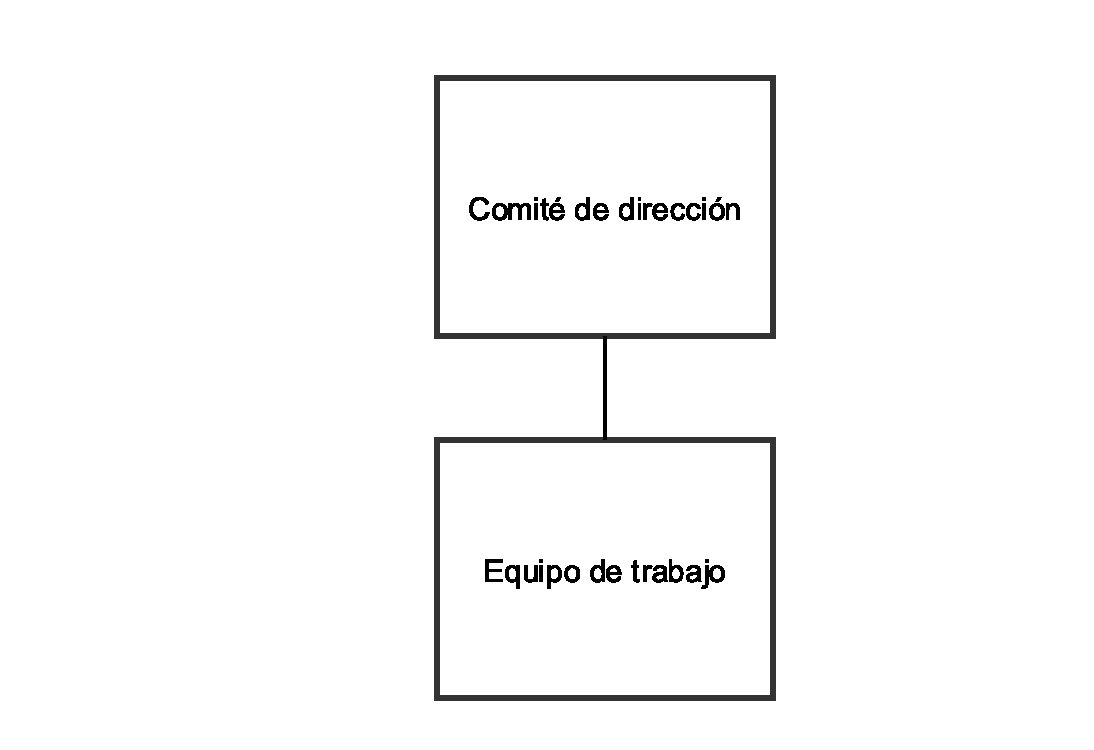
\includegraphics[scale=.75]{fig/organization}
	\caption{Esquema organizativo}
\end{figure}

\begin{itemize}
	\item Comité de dirección: su función principal es orientar por dónde debería ir el proyecto y tomar las decisiones finales a la hora de qué hacer o no.  Además, este comité deberá aprobar las diferentes fases del proyecto.
	\item Equipo de trabajo: el órgano encargado de diseñar y desarrollar el contenido del proyecto en función de las diferentes fases estipuladas.
\end{itemize}

\section{Plan de Recursos Humanos}

El equipo de trabajo estará formado por los siguientes perfiles directamente relacionados con las diferentes áreas de competencias que se abordan en el proyecto: 

\begin{itemize}
	\item Jefe de proyecto: su función es realizar las actividades de organización, coordinación y seguimiento del proyecto.
	\item Administrador de base de datos: su función es la de gestionar de una manera óptima la base de datos PostgreSQL y SPARQL y su función geoespacial. 
	\item Programador: su función es la desarrollar toda la lógica del programa como la implementación de la plataforma web. 
	\item Diseñador: su función es la diseñar interfaces intuitivas para el usuario y adaptables para distintos dispositivos (portátiles, tablets, móviles) 
	\item Experto en web semántica: su función es la de ayudar al equipo de trabajo a la hora de crear el sistema de búsquedas semánticas y facetadas. 
\end{itemize}

Debido a el bajo número de personas que compone el equipo de desarrollo se ha acordado trabajar mediante reuniones de seguimiento semanales pero también tras terminar cada tarea. En las reuniones semanales se reunirán todos los miembros del equipo, mientras que en las que corresponden a una tarea finalizada lo harán solo los que han participado en dicha tarea junto a el director de proyecto. Su finalidad será comentar los avances y/o problemas que hayan podido ocurrir, aunque también servirán para que el director de el visto bueno a la tarea y pasar a la siguiente. 

\chapter{Condiciones de ejecución}

\section{Entorno de trabajo}

El lugar de trabajo habitual serán las instalaciones de DeustoTech, aunque también se trabajará en casa para poder terminar a tiempo el proyecto.

El calendario y horario serán los correspondientes a los lugares de trabajo anteriormente mencionados durante una jornada laboral de aproximadamente 8 horas al día para los programadores, ya que este recurso es fundamental para el desarrollo del producto. Este horario podría verse modificado si se requiriera con el fin de cumplir los plazos establecidos.

En principio el director de proyecto será el responsable de todos los productos del desarrollo, y deberá dar el visto bueno a las herramientas que serán utilizadas para preservar las copias de seguridad y de definir cada cuanto tiempo deberán hacerse. En caso de que los desarrolladores no cumplan con estos requisitos y de producirse una perdida en el desarrollo serán estos los que asuman la responsabilidad, teniendo que optar por realizar horas extra o asumir de su sueldo la penalización que llegase a imponer el cliente en caso de no poder cumplirse con los plazos.

Los medios informáticos para la ejecución del proyecto deberán ser provistos por DeustoTech o serán los ordenadores personales de los integrantes del equipo. DeustoTech será responsable de todos los productos provistos para el desarrollo, salvo de aquellos medios pertenecientes a los propios desarrolladores. Los medios son los siguientes: 

\begin{itemize}
	\item Hardware
	\begin{itemize}
		\item Macbook Pro Retina 2012
		\item Servidor del repositorio Linux
		\item Monitor secundario
	\end{itemize}
	\item Software
	\begin{itemize}
		\item Licencia Sublime Text 2
		\item OS X
		\item Office 2011
		\item PostgreSQL
		\item SPARQL
	\end{itemize}
\end{itemize}

\section{Control de cambios}

Todas las peticiones que impliquen cambios en el diseño o en lo que ya está desarrollado, serán estudiadas y solo seguirán adelante si son modificaciones razonables y que son posibles de hacer dentro del plazo acordado. El procedimiento que habrá que seguir a la hora de  solicitar un cambio será:

\begin{enumerate}
	\item Comunicación de DeustoTech de las modificaciones solicitadas.
	\item Valoración por el equipo del proyecto de la repercusión técnica y cambios de plazos.
	\item Presentación de la decisión tomada por el equipo a DeustoTech.
	\item Notificación por parte de DeustoTech de la aprobación o no de la propuesta.	
	\item En caso afirmativo, modificación del plan de trabajo y del presupuesto.
\end{enumerate}

\section{Recepción de productos}

Para la recepción de productos el equipo del proyecto definirá una serie de pruebas que serán estrictamente ejecutadas. Una vez pasadas las pruebas, el jefe de proyecto deberá revisar y aceptar el producto para poder presentarlo oficialmente a DeustoTech.  En caso de que exista algún problema tras la revisión,  la dirección de DeustoTech-Internet deberá comunicarlo en un plazo máximo de 5 días para poder llevar a cabo las modificaciones y así poder seguir con la siguiente fase del proyecto. En caso de no obtener respuesta en el intervalo de tiempo especificado anteriormente, se considerará aprobado.

DeustoTech-Internet es el equipo de investigación centrado en el desarrollo web de la Universidad de Deusto. Este proyecto se ha delegado a varios de sus colaboradores de investigación. Dado a la estrecha relación que existen entre ambos no se han definido todos los requisitos desde el punto de partida, lo cual puede causar que retrasos en la fecha de entrega del producto. Sin embargo, al un proyecto interno no se le ha dado mayor importancia.

\chapter{Planificación}

\section{Diagrama de precedencias}

\section{Equipo}

\section{Plan de trabajo}

\section{Diagrama de Gantt}

\section{Estimación de cargas de trabajo por perfil}

\chapter{Presupuesto}

\section{Recursos Humanos}

\begin{center}
	\begin{tabular}{| l | r | r | r |}
		\hline
		Rol					&	Precio/hora(\euro/h)	&	Carga de trabajo(h)	&	Importe total(\euro)	\\	\hline
		Jefe de proyecto	& 	40						&	30 					& 	1.200					\\	\hline
		Administrador de base de datos &	25			&	158					&	3.950					\\	\hline
		Programador			&	25						&	520					&	13.000					\\	\hline
		Diseñador			&	15						&	82					&	1.230					\\	\hline
		Experto en web semántica	&		30			&	82					&	2.460					\\
		\hline
	\end{tabular}
\end{center}

\section{Recursos Software}

\begin{center}
	\begin{tabular}{| l | r | r | r |}
		\hline
		Nombre					&	Precio(\euro)	&	Unidades	&	Importe total(\euro)	\\	\hline
		Licencia Sublime Text 2	& 	70				&	1 			& 	70						\\	\hline
		Office 2011 			&	99				&	1			&	99						\\
		\hline
	\end{tabular}
\end{center}

\section{Recursos Hardware}

\begin{center}
	\begin{tabular}{| l | r | r | r |}
		\hline
		Nombre				&	Precio(\euro)	&	Unidades	&	Importe total(\euro)	\\	\hline
		MBPR2012			& 	3.334			&	2 			&	6.668					\\	\hline
		Monitor secundario	&	300				&	2			&	600						\\
		\hline
	\end{tabular}
\end{center}

\section{Total}

\begin{center}
	\begin{tabular}{| l | r |}
		\hline
		Tipo				&	Total			\\	\hline
		Recursos Humanos	& 	21.840			\\	\hline
		Recursos Software	&	169				\\	\hline
		Recursos Hardware	&	7.268			\\	\hline
		\textbf{Total}		&	\textbf{29.277}	\\
		\hline
	\end{tabular}
\end{center}